\documentclass[12pt,letterpaper]{article}

% ---------------------------------------------------------------------------
% Packages
% ---------------------------------------------------------------------------
\usepackage[margin=0.85in]{geometry}
\usepackage{newtxtext,newtxmath}
\usepackage{setspace}
\usepackage{titlesec}
\usepackage{booktabs}
\usepackage{array}
\usepackage{tabularx}
\usepackage{enumitem}
\usepackage{parskip}
\usepackage{microtype}
\usepackage[hidelinks]{hyperref}
\usepackage{fancyhdr}
\usepackage{tikz}
\usepackage{multirow}
\usetikzlibrary{shapes.geometric, arrows.meta, positioning, fit, backgrounds, calc}

% ---------------------------------------------------------------------------
% Page style
% ---------------------------------------------------------------------------
\pagestyle{fancy}
\fancyhf{}
\rhead{\small CIS 5690 -- Advanced Systems Project}
\lhead{\small SecureGate}
\rfoot{\small Page \thepage}
\renewcommand{\headrulewidth}{0.4pt}

% ---------------------------------------------------------------------------
% Section formatting
% ---------------------------------------------------------------------------
\titleformat{\section}{\large\bfseries}{}{0em}{}[\titlerule]
\titleformat{\subsection}{\normalsize\bfseries}{}{0em}{}
\titlespacing*{\section}{0pt}{12pt}{6pt}
\titlespacing*{\subsection}{0pt}{8pt}{4pt}

% ---------------------------------------------------------------------------
% Helpers
% ---------------------------------------------------------------------------
\newcolumntype{L}[1]{>{\raggedright\arraybackslash}p{#1}}
\newcolumntype{Y}{>{\raggedright\arraybackslash}X}

\setlength{\parindent}{0pt}
\setlength{\parskip}{4pt}
\setlength{\headheight}{14pt}
\setlist[itemize]{noitemsep, topsep=2pt, leftmargin=*, parsep=2pt}
\setlist[enumerate]{noitemsep, topsep=2pt, leftmargin=*, parsep=2pt}
\setstretch{1.10}

\begin{document}

% ---------------------------------------------------------------------------
% Title block
% ---------------------------------------------------------------------------
\begin{center}
    {\LARGE \textbf{SecureGate}} \\[4pt]
    {\large Course-Level Revision Plan and Structured System Report} \\[6pt]
    {\normalsize CIS 5690 -- Advanced Systems Project \quad | \quad Spring 2026} \\[2pt]
\end{center}
\vspace{2pt}
\hrule
\vspace{10pt}

% ---------------------------------------------------------------------------
\section{Executive Summary}

SecureGate is a deployed full-stack digital access-control platform that replaces manual gate registers and shareable identity cards with cryptographically signed QR passes, role-based approval workflows, optional face verification, geofence-aware pass generation, and real-time audit logging. The deployed baseline already demonstrates the end-to-end system flow across four portals: Member, Admin, Guard, and Contact.

After the demo review, the project requires a stronger course-level framing. The feedback indicates three main issues:
\begin{itemize}
    \item the use cases in the demo report are too implementation-centric and appear repetitive,
    \item GPS/geofence logic is repeated too often across the current write-up,
    \item the project needs one stronger scheduling or policy-driven feature to clearly reach course-project depth.
\end{itemize}

This revised report addresses those concerns by:
\begin{itemize}
    \item restructuring the project around \textbf{12 distinct actor-goal use cases},
    \item consolidating GPS into only two places: \textbf{instant on-campus pass generation} and \textbf{admin policy configuration},
    \item implementing \textbf{slot-based access scheduling} as the primary course-level enhancement,
    \item clearly separating the original deployed baseline from the completed course-level extension,
    \item presenting a realistic hardening, testing, and documentation plan.
\end{itemize}

% ---------------------------------------------------------------------------
\section{Feedback-Driven Revision Strategy}

\begin{tabularx}{\textwidth}{@{}L{4.2cm}Y Y@{}}
\toprule
\textbf{Observed Demo Feedback} & \textbf{Revision Decision in This Report} & \textbf{Expected Impact} \\
\midrule
Use cases felt too similar & Rewrite the system around 12 actor-centered, goal-based use cases instead of feature-only descriptions & Stronger academic clarity and better problem-to-solution mapping \\
GPS appeared repeatedly in the report & Limit GPS to UC06 (instant on-campus pass) and UC11 (policy and boundary configuration) & Removes redundancy and makes the use-case set more distinct \\
Need stronger course-level depth & Implement slot-based access scheduling with capacity, time-window, and policy enforcement & Adds a clear systems-design extension beyond the original deployment \\
Documentation overstated or mixed implemented and planned work & Split the report into original baseline, completed extension, and remaining hardening & More professional and defensible during evaluation \\
Need reasonable scope in short time & Prioritize one high-value extension plus analytics, testing, and demo alignment & Keeps the project ambitious but still finishable \\
\bottomrule
\end{tabularx}

% ---------------------------------------------------------------------------
\section{Current Deployed Baseline}

The currently deployed build already supports the following operational capabilities:
\begin{itemize}
    \item access-request workflow with admin approval,
    \item JWT authentication and role-based access control,
    \item QR pass generation with HMAC-based integrity protection,
    \item standard pass request and approval flow,
    \item instant daily entry or exit pass generation,
    \item guard-side camera QR scanning and verification,
    \item optional face registration and gate-side face comparison,
    \item geofence-aware location validation,
    \item admin dashboard with pass queue and real-time logs,
    \item contact or parent history view through a signed access link,
    \item emergency exit workflow,
    \item Render deployment with Docker-based hosting.
\end{itemize}

The original baseline was already a valid working system. The completed revision adds the stronger scheduling and policy layer needed for a cleaner course-level submission.

% ---------------------------------------------------------------------------
\section{Revised Course-Level Scope}

\textbf{Project objective:} transform SecureGate from a functional gate-pass prototype into a policy-driven access-control system suitable for course evaluation in distributed systems, backend architecture, and access-governance design.

\textbf{In-scope revision goals:}
\begin{itemize}
    \item redesign the report around distinct use cases,
    \item implement slot-based access scheduling,
    \item bind selected passes to slot windows and capacity constraints,
    \item strengthen administrative analytics,
    \item add formal testing, requirements, and UML artifacts,
    \item align the deployed build, the report, and the demo script.
\end{itemize}

\textbf{Out-of-scope for this milestone:}
\begin{itemize}
    \item native mobile applications,
    \item Kubernetes-scale deployment,
    \item anomaly-detection machine learning,
    \item RFID or NFC hardware integration.
\end{itemize}

% ---------------------------------------------------------------------------
\section{Revised System Architecture}

\begin{center}
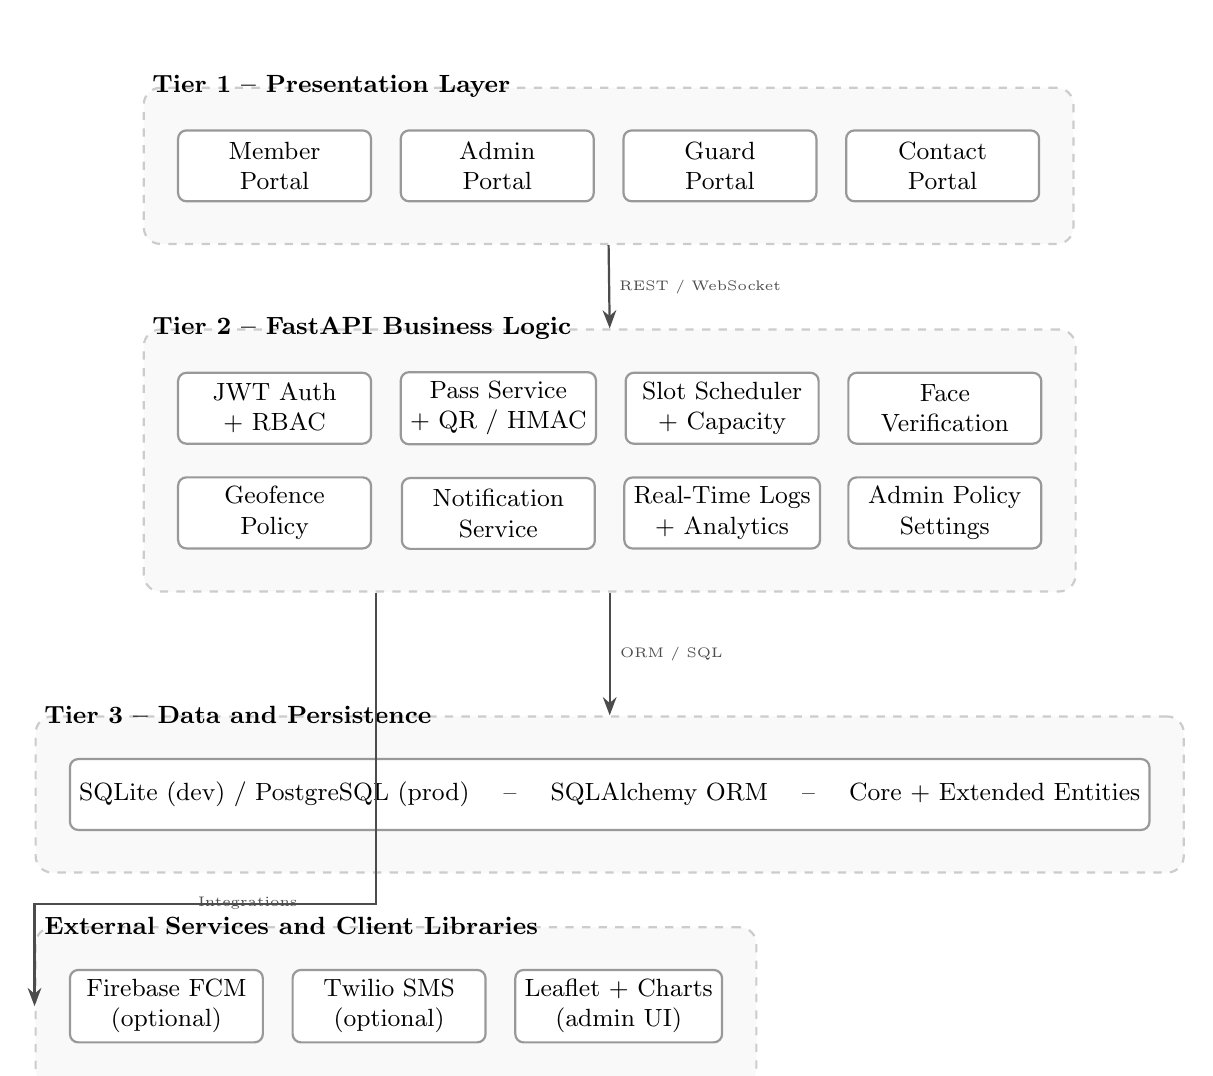
\begin{tikzpicture}[
    node distance=1.05cm and 0.35cm,
    every node/.style={font=\small},
    mybox/.style={
        rectangle, draw=gray!80, thick,
        rounded corners=3pt,
        minimum width=2.45cm, minimum height=0.9cm,
        align=center, fill=white
    },
    tierbox/.style={
        rectangle, draw=gray!40, dashed, thick,
        rounded corners=6pt, fill=gray!5,
        inner xsep=12pt, inner ysep=15pt
    },
    arrow/.style={-Stealth, thick, black!70}
]

% Tier 1
\node[mybox] (mp) {Member\\Portal};
\node[mybox, right=of mp] (ad) {Admin\\Portal};
\node[mybox, right=of ad] (gd) {Guard\\Portal};
\node[mybox, right=of gd] (cp) {Contact\\Portal};

\begin{pgfonlayer}{background}
  \node[tierbox, fit=(mp)(ad)(gd)(cp)] (T1) {};
\end{pgfonlayer}
\node[font=\small\bfseries, anchor=west] at (T1.north west) {Tier 1 -- Presentation Layer};

% Tier 2
\node[mybox, below=2.15cm of mp] (auth) {JWT Auth\\+ RBAC};
\node[mybox, right=of auth] (pass) {Pass Service\\+ QR / HMAC};
\node[mybox, right=of pass] (slot) {Slot Scheduler\\+ Capacity};
\node[mybox, right=of slot] (face) {Face\\Verification};

\node[mybox, below=0.4cm of auth] (geo) {Geofence\\Policy};
\node[mybox, below=0.4cm of pass] (notif) {Notification\\Service};
\node[mybox, below=0.4cm of slot] (rt) {Real-Time Logs\\+ Analytics};
\node[mybox, below=0.4cm of face] (settings) {Admin Policy\\Settings};

\begin{pgfonlayer}{background}
  \node[tierbox, fit=(auth)(pass)(slot)(face)(geo)(notif)(rt)(settings)] (T2) {};
\end{pgfonlayer}
\node[font=\small\bfseries, anchor=west] at (T2.north west) {Tier 2 -- FastAPI Business Logic};

% Tier 3
\node[mybox, minimum width=11.1cm, below=2.1cm of T2] (db)
    {SQLite (dev) / PostgreSQL (prod) \quad -- \quad SQLAlchemy ORM \quad -- \quad Core + Extended Entities};

\begin{pgfonlayer}{background}
  \node[tierbox, fit=(db)] (T3) {};
\end{pgfonlayer}
\node[font=\small\bfseries, anchor=west] at (T3.north west) {Tier 3 -- Data and Persistence};

% External Services
\node[mybox, below=1.75cm of db.south west, anchor=north west] (fcm) {Firebase FCM\\(optional)};
\node[mybox, right=of fcm] (twilio) {Twilio SMS\\(optional)};
\node[mybox, right=of twilio] (ui) {Leaflet + Charts\\(admin UI)};

\begin{pgfonlayer}{background}
  \node[tierbox, fit=(fcm)(twilio)(ui)] (T4) {};
\end{pgfonlayer}
\node[font=\small\bfseries, anchor=west] at (T4.north west) {External Services and Client Libraries};

% Connectors
\draw[arrow] (T1.south) -- (T2.north) node[midway, right, font=\tiny] {REST / WebSocket};
\draw[arrow] (T2.south) -- (T3.north) node[midway, right, font=\tiny] {ORM / SQL};
\draw[arrow] ($(T2.south west)!0.25!(T2.south east)$) -- ++(0,-3.95) -| (T4.west) node[pos=0.1, left, font=\tiny] {Integrations};

\end{tikzpicture}
\end{center}

\textbf{Persisted entities:}
\begin{itemize}
    \item \texttt{users}
    \item \texttt{registration\_requests}
    \item \texttt{passes}
    \item \texttt{scan\_logs}
    \item \texttt{slots} -- time window, gate, capacity, policy flags
    \item \texttt{slot\_bookings} -- user-slot reservation and status history
\end{itemize}

% ---------------------------------------------------------------------------
\section{Actors and Responsibilities}

\begin{tabularx}{\textwidth}{@{}L{2cm}L{2.8cm}Y@{}}
\toprule
\textbf{Actor} & \textbf{Interface} & \textbf{Responsibility} \\
\midrule
Member & Member Portal & Request access, reserve slots, request standard passes, generate instant on-campus passes, maintain profile, trigger emergency exit \\
Admin & Admin Portal & Approve accounts and passes, define slot schedules, configure geofence and policy, monitor operations, review analytics \\
Guard & Guard Portal & Scan QR codes, verify face for restricted entries, enforce slot windows, log exceptions at the checkpoint \\
Contact & Contact Portal & View recent movement history through signed link access and receive alert subscriptions \\
Visitor & Admin-mediated flow & Receive one-time or scheduled guest access through host or admin provisioning \\
\bottomrule
\end{tabularx}

% ---------------------------------------------------------------------------
\section{Reframed Use Cases}

This revised set intentionally limits GPS-specific logic to only two use cases: UC06 and UC11. The remaining use cases focus on different actors, policies, and system goals.

\subsection{UC01 -- Access Request Submission}
\textbf{Primary actor:} Member applicant

\textbf{Goal:} Request system access for authorized use.

\textbf{Preconditions:}
\begin{itemize}
    \item The applicant does not yet have an active account.
\end{itemize}

\textbf{Main flow:}
\begin{enumerate}
    \item The applicant opens the Member Portal and fills in identity and role details.
    \item The system validates email, personnel ID, and request completeness.
    \item A pending \texttt{registration\_request} record is created.
    \item Admin users are notified that a new account request is awaiting review.
\end{enumerate}

\textbf{Alternate flow:}
\begin{itemize}
    \item If the email or personnel ID already exists, the request is rejected immediately.
    \item If another pending request already exists, the system prevents duplicate submission.
\end{itemize}

\textbf{Postconditions:} A pending access request is stored and visible in the admin queue.

\subsection{UC02 -- Account Review and Provisioning}
\textbf{Primary actor:} Admin

\textbf{Goal:} Approve or reject a pending account request and provision the correct role.

\textbf{Preconditions:}
\begin{itemize}
    \item An admin is authenticated.
    \item At least one pending registration request exists.
\end{itemize}

\textbf{Main flow:}
\begin{enumerate}
    \item The admin reviews submitted identity details and requested role.
    \item The admin approves the request and optionally adjusts the final role.
    \item The system creates the user record and activates login access.
    \item The request record is updated with review metadata and linked to the created account.
\end{enumerate}

\textbf{Alternate flow:}
\begin{itemize}
    \item The admin rejects the request and records a review note.
\end{itemize}

\textbf{Postconditions:} The request is permanently marked approved or rejected, and the user account state is synchronized.

\subsection{UC03 -- Slot Definition and Capacity Planning}
\textbf{Primary actor:} Admin

\textbf{Goal:} Define controlled entry or exit windows for members and visitors.

\textbf{Preconditions:}
\begin{itemize}
    \item The admin is authenticated.
\end{itemize}

\textbf{Main flow:}
\begin{enumerate}
    \item The admin creates a slot with label, gate, start time, end time, and maximum capacity.
    \item The admin optionally enables policy flags such as GPS-required or face-check-required.
    \item The slot is saved and published to eligible users.
    \item The dashboard shows remaining capacity and slot status.
\end{enumerate}

\textbf{Alternate flow:}
\begin{itemize}
    \item Invalid time ranges or zero capacity are rejected at validation time.
    \item Overlapping administrative policies can be flagged for review.
\end{itemize}

\textbf{Postconditions:} A slot definition is available for booking and policy enforcement.

\subsection{UC04 -- Slot Booking by Member}
\textbf{Primary actor:} Member

\textbf{Goal:} Reserve an approved access window before reaching the gate.

\textbf{Preconditions:}
\begin{itemize}
    \item The member account is active.
    \item At least one eligible slot is available.
\end{itemize}

\textbf{Main flow:}
\begin{enumerate}
    \item The member views available slots in the portal.
    \item The member selects a slot matching the intended entry or exit time.
    \item The system checks capacity, duplication, and role restrictions.
    \item A \texttt{slot\_booking} record is created and linked to the eventual pass flow.
\end{enumerate}

\textbf{Alternate flow:}
\begin{itemize}
    \item If the slot is full, the booking is rejected and the user is asked to choose another slot.
    \item If the member already holds a conflicting reservation, the duplicate booking is blocked.
\end{itemize}

\textbf{Postconditions:} The member has a reserved access window recorded in the system.

\subsection{UC05 -- Standard Pass Request with Admin Approval}
\textbf{Primary actor:} Member

\textbf{Goal:} Request a non-urgent pass that still requires administrative approval.

\textbf{Preconditions:}
\begin{itemize}
    \item The member is authenticated.
\end{itemize}

\textbf{Main flow:}
\begin{enumerate}
    \item The member submits reason, pass type, and optional supporting data.
    \item The system creates a pending pass request.
    \item Admin users review the request and approve or reject it.
    \item On approval, the system generates a time-limited HMAC-signed QR token.
\end{enumerate}

\textbf{Alternate flow:}
\begin{itemize}
    \item Rejection returns a final status and optional review feedback.
\end{itemize}

\textbf{Postconditions:} The pass is either rejected or converted into an approved QR-based credential.

\subsection{UC06 -- Instant On-Campus Pass Generation}
\textbf{Primary actor:} Member

\textbf{Goal:} Generate an immediate pass from inside the configured campus boundary.

\textbf{Preconditions:}
\begin{itemize}
    \item The member is authenticated.
    \item Browser geolocation is available.
\end{itemize}

\textbf{Main flow:}
\begin{enumerate}
    \item The member requests an instant entry or exit pass.
    \item The client captures latitude and longitude from the browser geolocation API.
    \item The server validates distance to the configured campus boundary with the allowed GPS buffer.
    \item If valid, the pass is auto-approved and the QR token is generated immediately.
\end{enumerate}

\textbf{Alternate flow:}
\begin{itemize}
    \item If the location is outside the boundary, the request is denied.
    \item If GPS permission is unavailable, the user falls back to the standard approval path.
\end{itemize}

\textbf{Postconditions:} A geofence-compliant instant pass is issued or the request is denied.

\subsection{UC07 -- Visitor Pass Creation}
\textbf{Primary actor:} Admin

\textbf{Goal:} Issue one-time or scheduled access to an external guest.

\textbf{Preconditions:}
\begin{itemize}
    \item The admin is authenticated.
    \item Visitor identity or host details are available.
\end{itemize}

\textbf{Main flow:}
\begin{enumerate}
    \item The admin enters visitor details, validity period, and optional assigned slot.
    \item The system creates a restricted pass with a short validity window.
    \item A QR token is generated and shared to the visitor through the approved channel.
    \item The guard sees the visitor flag during verification.
\end{enumerate}

\textbf{Alternate flow:}
\begin{itemize}
    \item If the requested window conflicts with policy or capacity, the visitor pass is not issued.
\end{itemize}

\textbf{Postconditions:} A visitor credential is issued with tighter policy controls than a normal member pass.

\subsection{UC08 -- QR Verification at the Checkpoint}
\textbf{Primary actor:} Guard

\textbf{Goal:} Validate a presented QR pass before allowing entry or exit.

\textbf{Preconditions:}
\begin{itemize}
    \item A guard is authenticated.
    \item The member or visitor presents a QR token.
\end{itemize}

\textbf{Main flow:}
\begin{enumerate}
    \item The guard scans or pastes the QR token.
    \item The system parses the token and recomputes the HMAC signature.
    \item The system checks expiry, pass state, one-time-use status, and slot window if applicable.
    \item On success, the pass is marked used and a scan log entry is created.
\end{enumerate}

\textbf{Alternate flow:}
\begin{itemize}
    \item Signature mismatch produces an invalid-token rejection.
    \item Expired or already-used passes are denied and logged.
    \item Slot-window mismatch is denied with an explanatory message.
\end{itemize}

\textbf{Postconditions:} The checkpoint outcome is committed to the audit log and reflected in dashboards.

\subsection{UC09 -- Restricted Access Face Verification}
\textbf{Primary actor:} Guard

\textbf{Goal:} Confirm identity for entries that require stronger proof than QR alone.

\textbf{Preconditions:}
\begin{itemize}
    \item The presented pass is valid.
    \item The access policy requires face verification or the guard manually enables it.
\end{itemize}

\textbf{Main flow:}
\begin{enumerate}
    \item The guard captures a live face image after the QR is accepted.
    \item The system extracts the live encoding and compares it with the enrolled template.
    \item Confidence and match status are computed.
    \item The guard is shown a clear allow or deny result with reason.
\end{enumerate}

\textbf{Alternate flow:}
\begin{itemize}
    \item If no face is enrolled, the system records the condition and triggers fallback handling.
    \item If the image is poor or no face is detected, the verification is retried or denied.
\end{itemize}

\textbf{Postconditions:} Identity-sensitive access decisions become auditable and policy-driven.

\subsection{UC10 -- Contact Subscription and History Review}
\textbf{Primary actor:} Contact

\textbf{Goal:} View recent movement history and subscribe to future alerts without a full account.

\textbf{Preconditions:}
\begin{itemize}
    \item The contact receives a signed access link from the member.
\end{itemize}

\textbf{Main flow:}
\begin{enumerate}
    \item The contact opens the signed link.
    \item The system validates the signed token and maps it to the correct member record.
    \item The contact sees recent successful entry and exit history.
    \item Optional phone number and notification token are saved for future alerts.
\end{enumerate}

\textbf{Alternate flow:}
\begin{itemize}
    \item Invalid or expired signed links are rejected.
\end{itemize}

\textbf{Postconditions:} The contact can monitor movement history without being provisioned as a full user.

\subsection{UC11 -- Live Monitoring and Policy Adjustment}
\textbf{Primary actor:} Admin

\textbf{Goal:} Monitor operations in real time and refine access policy from the control dashboard.

\textbf{Preconditions:}
\begin{itemize}
    \item The admin is authenticated.
\end{itemize}

\textbf{Main flow:}
\begin{enumerate}
    \item The admin opens the dashboard and receives live WebSocket updates.
    \item The system shows recent scans, hourly counts, daily trends, and error conditions.
    \item The admin adjusts policy settings such as geofence center, radius, or slot availability.
    \item Updated settings become active for future requests.
\end{enumerate}

\textbf{Alternate flow:}
\begin{itemize}
    \item If live WebSocket delivery is unavailable, the dashboard falls back to polling-based refresh.
\end{itemize}

\textbf{Postconditions:} Administrative awareness and policy control remain synchronized with gate activity.

\subsection{UC12 -- Emergency Exit Handling}
\textbf{Primary actor:} Member

\textbf{Goal:} Exit the secured area immediately during an urgent situation.

\textbf{Preconditions:}
\begin{itemize}
    \item The member is authenticated.
\end{itemize}

\textbf{Main flow:}
\begin{enumerate}
    \item The member triggers an emergency exit request from the portal.
    \item The system records an emergency scan log entry without waiting for pass approval.
    \item Admin users are notified about the emergency event.
    \item The event appears in real-time logs for oversight.
\end{enumerate}

\textbf{Alternate flow:}
\begin{itemize}
    \item Notification delivery failure does not cancel the emergency record or exit approval.
\end{itemize}

\textbf{Postconditions:} The emergency action is granted quickly while preserving a full audit trail.

% ---------------------------------------------------------------------------
\section{Data Model Revision}

\small
\begin{tabularx}{\textwidth}{@{}L{3.4cm}L{3.6cm}Y@{}}
\toprule
\textbf{Entity} & \textbf{Key Fields} & \textbf{Purpose} \\
\midrule
\texttt{users} & id, role, member ID, face fields, contact fields, validity & Identity, role, and notification ownership \\
\shortstack[l]{\texttt{registration\_}\\\texttt{requests}} & requester details, requested role, review status, reviewer metadata & Access provisioning workflow \\
\texttt{passes} & user ID, reason, pass type, status, QR token, expiry, usage fields & Access credential lifecycle \\
\texttt{scan\_logs} & pass ID, scanner ID, result, pass type, details, emergency & Immutable audit history \\
\texttt{slots} & label, gate, start/end time, capacity, active, policy flags & Time-window and capacity definition \\
\texttt{slot\_bookings} & slot ID, user ID, pass ID, booking status, booked at & Reservation and allocation history \\
\bottomrule
\end{tabularx}
\normalsize

Implemented pass extensions:
\begin{itemize}
    \item \texttt{passes.slot\_id} to bind a pass to a reserved slot,
    \item \texttt{passes.access\_mode} to distinguish standard, instant, slot-bound, and visitor flows,
    \item \texttt{passes.requires\_face\_check} where policy requires stronger verification.
\end{itemize}

% ---------------------------------------------------------------------------
\section{Technology Stack}

\begin{tabularx}{\textwidth}{@{}L{3.3cm}L{1.8cm}Y@{}}
\toprule
\textbf{Technology} & \textbf{Version} & \textbf{Role in the Revised Project} \\
\midrule
Python & 3.11+ & Core backend language \\
FastAPI & 0.115.x & REST API, dependency injection, request validation, async endpoints \\
Uvicorn & 0.30.x & ASGI server for HTTP and WebSocket transport \\
SQLAlchemy & 2.0.x & ORM and persistence layer across SQLite and PostgreSQL \\
Pydantic + pydantic-settings & 2.x & Schema validation and environment-based configuration \\
PyJWT & 2.9.x & JWT authentication and signed contact-link tokens \\
Passlib + bcrypt & 1.7.x & Password hashing and verification \\
HMAC-SHA256 & stdlib & Tamper-proof QR signature generation and verification \\
OpenCV & 4.8.x & Default lightweight image processing and face feature extraction \\
face-recognition & optional & Alternate heavier face backend when explicitly enabled \\
Pillow & 10.x & Image validation and normalization \\
geopy & 2.4.x & Geodesic distance checks for campus boundary validation \\
Shapely & 2.0.x & Polygon-based geofence support \\
firebase-admin & 6.3.x & Optional server-side push notifications \\
Twilio & 8.10.x & Optional SMS delivery \\
APScheduler & 3.10.x & Background scheduling and future analytics jobs \\
jsQR & CDN & In-browser QR scanning in the Guard Portal \\
QRCode.js & CDN & Client-side QR rendering \\
Chart.js & CDN & Dashboard charts for analytics and trends \\
Leaflet.js & CDN & Interactive map for geofence and policy setup \\
\bottomrule
\end{tabularx}

% ---------------------------------------------------------------------------
\section{Deployed Baseline vs Course-Level Target}

\begin{tabularx}{\textwidth}{@{}L{3.4cm}Y Y@{}}
\toprule
\textbf{Dimension} & \textbf{Original Baseline} & \textbf{Completed Revision} \\
\midrule
Use-case framing & Feature-driven and partly repetitive in the earlier report & Actor-centered, 12 distinct use cases \\
Access decision & QR, approval state, optional face, geofence-aware instant pass & Policy-driven QR + slot + face + time-window enforcement \\
Scheduling & No explicit slot reservation & Slot creation, booking, pass binding, capacity, and time-window validation \\
Analytics & Live logs and dashboard counts & Historical trend, compliance rate, slot utilization, export endpoints \\
Documentation & Demo report exists & Final report, UML, requirements, test plan, polished demo script \\
Testing & Minimal ad hoc verification & Structured unit and integration test coverage \\
\bottomrule
\end{tabularx}

% ---------------------------------------------------------------------------
\section{Implementation Status and Hardening Plan}

\subsection{Phase 1 -- Documentation and Scope Alignment}
\begin{itemize}
    \item finalize the revised system story and actor-goal use cases,
    \item update terminology so the report, UI, and backend role names stay consistent,
    \item prepare UML and requirements around the revised scope.
\end{itemize}

\subsection{Phase 2 -- Slot-Based Access Scheduling}
\begin{itemize}
    \item implemented \texttt{slots} and \texttt{slot\_bookings} schema support,
    \item built admin slot creation and capacity management,
    \item added member slot booking and slot-bound pass requests,
    \item enforced slot window checks during guard verification.
\end{itemize}

\subsection{Phase 3 -- Analytics, Testing, and Hardening}
\begin{itemize}
    \item add analytics endpoints for peak hours, trend lines, and compliance metrics,
    \item create pytest coverage for crypto, auth, geofence, and slot logic,
    \item harden production settings such as CORS and event-loop handling,
    \item align the deployed demo with the revised report and final presentation flow.
\end{itemize}

\subsection{Immediate Finalization Priority Plan}
\begin{tabularx}{\textwidth}{@{}L{1.5cm}Y@{}}
\toprule
\textbf{Day} & \textbf{Priority Deliverables} \\
\midrule
Day 1 & verify all four portals, slot-bound pass approval, visitor QR, guardian link, and guard verification \\
Day 2 & polish analytics views, regenerate documentation PDFs, rerun tests, update demo flow, redeploy \\
\bottomrule
\end{tabularx}

% ---------------------------------------------------------------------------
\section{Testing and Evaluation Plan}

\textbf{Core automated tests to add:}
\begin{itemize}
    \item \texttt{test\_crypto.py}: token generation, tamper detection, expiry behavior, replay protection
    \item \texttt{test\_auth.py}: valid login, invalid password, inactive user, role enforcement
    \item \texttt{test\_geofence.py}: inside, outside, invalid coordinates, buffer zone, policy-disabled mode
    \item \texttt{test\_slot\_scheduler.py}: capacity limit, double booking, expired slot, slot-bound verification
    \item \texttt{test\_face\_auth.py}: enrollment status, match, mismatch, degraded image handling
\end{itemize}

\textbf{Evaluation metrics for the final project:}
\begin{itemize}
    \item QR verification success rate,
    \item average checkpoint verification time,
    \item percentage of denied replay attempts,
    \item slot utilization percentage,
    \item geofence compliance rate for instant passes,
    \item alert-delivery success ratio when notification providers are configured.
\end{itemize}

% ---------------------------------------------------------------------------
\section{Professional Submission Positioning}

For the final course submission, SecureGate should be presented as:
\begin{itemize}
    \item a \textbf{deployed baseline system} that already demonstrates real access-control flows,
    \item a \textbf{course-level revision} that introduces slot-based policy enforcement,
    \item a \textbf{distributed systems project} with multi-portal coordination, real-time logs, cryptographic verification, and configurable operational policy.
\end{itemize}

This positioning is stronger than simply claiming many isolated technical features, because it demonstrates:
\begin{itemize}
    \item problem decomposition,
    \item policy-aware system design,
    \item realistic incremental engineering,
    \item honest separation of implemented and planned work,
    \item a coherent path from prototype to course-quality system.
\end{itemize}

% ---------------------------------------------------------------------------
\section{Conclusion}

The revised SecureGate report turns the project into a cleaner, more defensible course submission. Instead of repeating GPS-heavy or implementation-only use cases, it now emphasizes distinct user goals, policy-driven access control, and a concrete systems extension through slot scheduling. This makes the next development steps clear:
\begin{enumerate}
    \item keep the deployed baseline stable,
    \item demonstrate slot-based scheduling and enforcement,
    \item strengthen analytics, tests, and formal project documentation,
    \item present the final project as a structured access-control platform rather than only a gate-pass demo.
\end{enumerate}

\end{document}
